%!TEX root = ../template.tex

\chapter{Validation and Experimental Evaluation}
\label{cha:validation_experimental_Evaluation}

This chapter presents, analyses and discusses the work performed to obtain relevant evaluation criteria measured from the complete system deployed on a cloud environment in order to validate the implemented prototype.

Section \ref{sec:testbench_environment} details how the system is deployed, explains the different configurations that that system adopts in order to present relevant data to compare.

In section \ref{sec:benchmarks_and_revelant_evaluation_criteria} explains which metrics will be evaluated for each different testbench scenario. Sections \ref{sec:performance_evaluation_redis_benchmark_tool} through \ref{sec:complementary_measurements} presents the actual metrics taken from the performance and load testing tools and compares the different system configurations with secure and vulnerable storage instances.

The last section, section \ref{sec:summary_and_findings} contains a summary of all the finding and some considerations that can be taken from the presented metrics.

\section{Testbench Environments}
\label{sec:testbench_environment}

There are multiple testbenchs, redis-benchmark for standalone instance, proxy with standalone instance for both secure and unsecure redis configurations, proxy with cluster for both secure and unsecure redis configurations, homomorphic operations for standalone instance, attestation operations, both sgx attestation at startup and software attestation on demand.

Talk about how the systems are deployed on the multiple testbenchs.

\section{Benchmarks and Relevant Evaluation Criteria}
\label{sec:benchmarks_and_revelant_evaluation_criteria}

Latency, throughputs, startup times, memory and cpu consumptions.

\section{Performance evaluation for Redis-Benchmark tool}
\label{sec:performance_evaluation_redis_benchmark_tool}

\begin{figure}[htbp]
  \centering
  \subcaptionbox{Redis Latency External\label{fig:redis_latency_external_2}}%
    {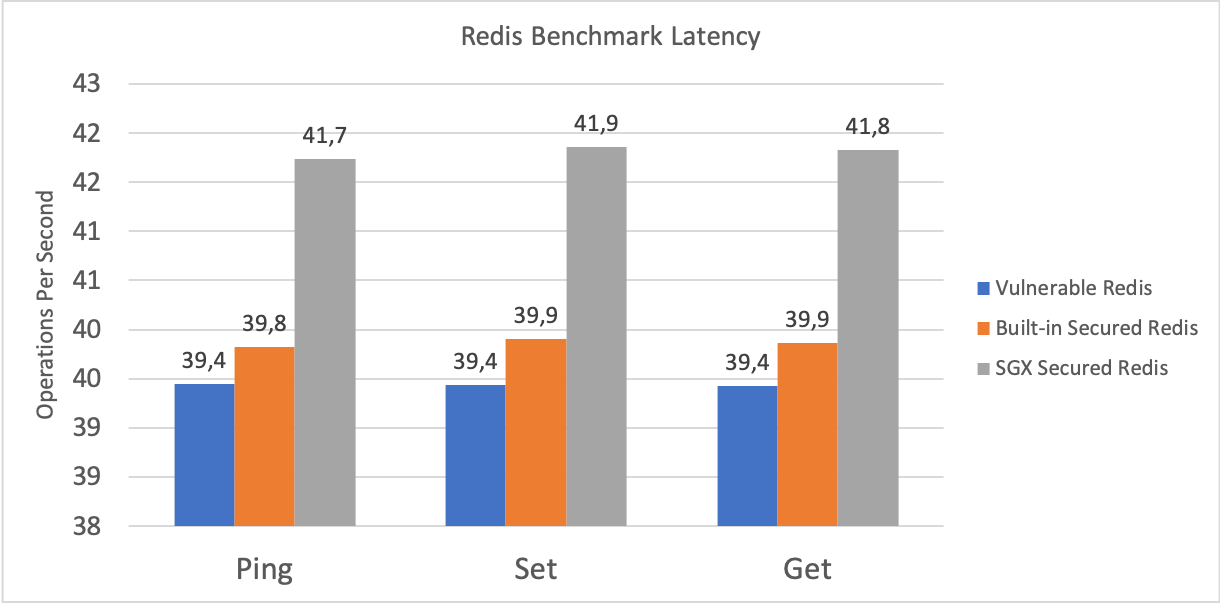
\includegraphics[width=0.5\linewidth]{redis_latency_external_2}}%
    %\hspace{1em}
  \subcaptionbox{Redis Throughput External\label{fig:redis_throughput_external_2}}%
    {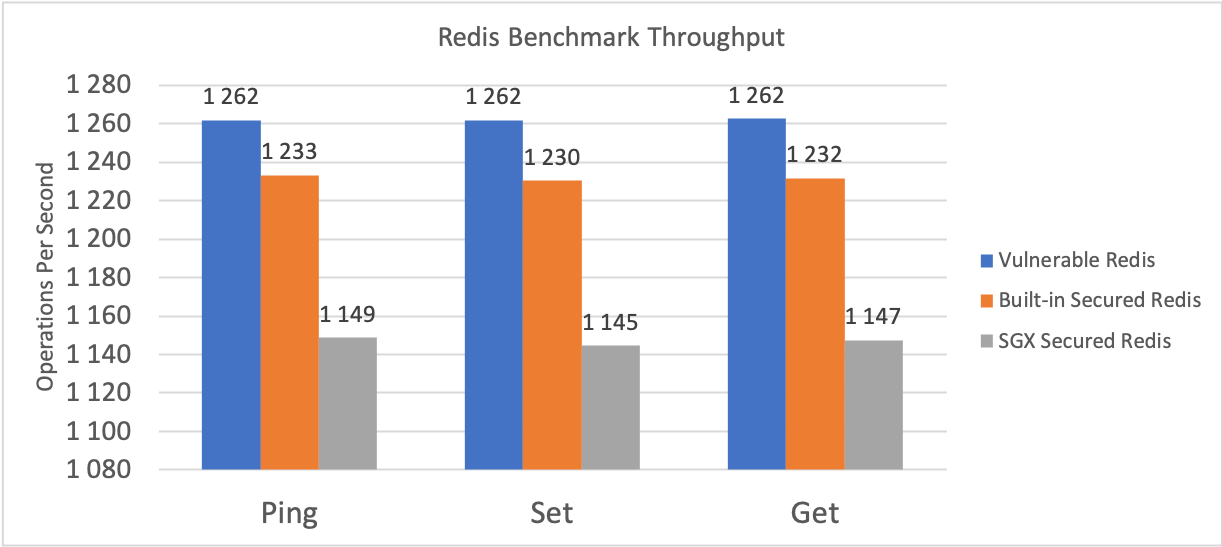
\includegraphics[width=0.5\linewidth]{redis_throughput_external_2}}%
  \caption{Redis Benchmark External Client Metrics}
  \label{fig:redis_benchmark_external_metrics}
\end{figure}

\begin{figure}[htbp]
  \centering
  \subcaptionbox{Redis Latency Internal\label{fig:redis_latency_internal}}%
    {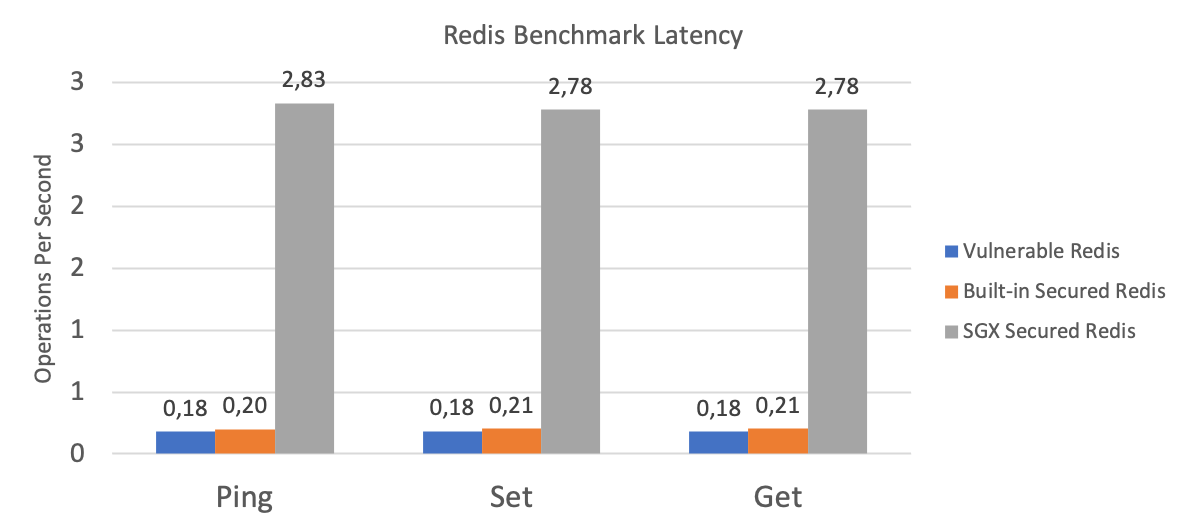
\includegraphics[width=0.5\linewidth]{redis_latency_internal}}%
    %\hspace{1em}
  \subcaptionbox{Redis Throughput Internal\label{fig:redis_throughput_internal}}%
    {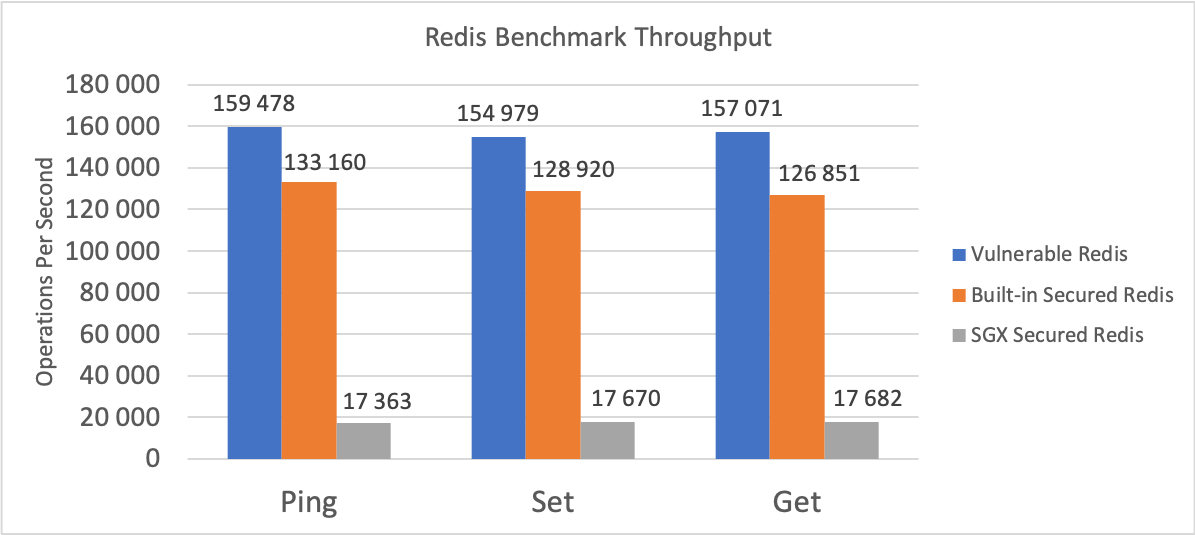
\includegraphics[width=0.5\linewidth]{redis_throughput_internal}}%
  \caption{Redis Benchmark Internal Client Metrics}
  \label{fig:redis_benchmark_internal_metrics}
\end{figure}


\section{Performance evaluation for Standalone Redis}
\label{sec:performance_evaluation_standalone_redis}

\section{Performance evaluation for Cluster Redis}
\label{sec:performance_evaluation_cluster_redis}

\section{Performance evaluation for Homomorphic Operations}
\label{sec:performance_evaluation_homomorphic_operations}

\section{Evaluation of the Attestation Protocol}
\label{sec:evaluation_attestation_protocol}

Get startup times with and without CAS, get stack attestation times...

\section{Complementary Measurements}
\label{sec:complementary_measurements}

Memory, CPU, etc instrumentation, workload

\section{ Summary and Findings}
\label{sec:summary_and_findings}

% \section{Performance evaluation for Testbench 1}
% \label{sec:performance_evaluation_testbench_1}

% \subsection{Latency}
% \label{ssec:testbench_1_latency}

% \subsection{Throughput}
% \label{ssec:testbench_1_throughput}

% \section{Performance evaluation for Testbench 2}
% \label{sec:performance_evaluation_testbench_2}

% \subsection{Latency}
% \label{ssec:testbench_2_latency}

% \subsection{Throughput}
% \label{ssec:testbench_2_throughput}

% \section{Evaluation of the Attestation Protocol}
% \label{sec:evaluation_attestation_protocol}

% Get startup times with and without CAS, get stack attestation times...

% \section{Complementary Measurements}
% \label{sec:complementary_measurements}

% Memory, CPU, etc instrumentation, workload

% \section{ Summary and Findings}
% \label{sec:summary_and_findings}
